\subsection{Sparse matrices}

A \definitionWithSpecificIndex{sparse matrix}{Sparse Matrix} is a matrix in which most of the elements are zero; roughly speaking, given $A \in \mathbb{R}^{n \times n}$, the number of non-zero entries of $A$ (denoted $\nnz\left(A\right)$) is $O\left(n\right)$, we say that $A$ is \textbf{sparse}.

\highspace
Sparse matrices are so important because when we try to solve:
\begin{equation*}
	A \mathbf{x} = \mathbf{b}
\end{equation*}
The $A$ matrix is often sparse, especially when it comes from the discretization of partial differential equations.

\highspace
Finally, note that the iterative methods (explained in the next section) only use a sparse matrix $A$ in the context of the matrix-vector product. Then we only need to provide the matrix-vector product to the computer.

\longline

\subsubsection{Storage schemes}

Unfortunately, storing a sparse matrix is a waste of memory. Instead of storing a dense array (with many zeros), the main idea is to \textbf{store only the non-zero entries, plus their locations}.

\highspace
This technique allows to save data storage because it will be from $O\left(n^{2}\right)$ to $O\left(\nnz\right)$.

\highspace
The most common sparse storage types are:
\begin{itemize}
	\item \definition{Coordinate format (COO)}. The data structure consists of three arrays (of length $\nnz\left(A\right)$):
	\begin{itemize}
		\item \texttt{AA}: all the values of the non-zero elements of $A$ in any order.
		
		\item \texttt{JR}: integer array containing their row indices.
		
		\item \texttt{JC}: integer array containing their column indices.
	\end{itemize}
	For \example{example}:
	\begin{equation*}
		A = \begin{bmatrix}
			1. & 0. & 0.& 2. & 0. \\
			3. & 4. & 0.& 5. & 0. \\
			6. & 0. & 7.& 8. & 9. \\
			0. & 0. & 10.& 11. & 0. \\
			0. & 0. & 0.& 0. & 12. 
		\end{bmatrix}
	\end{equation*}
	\begin{equation*}
		\begin{array}{rcl}
			\texttt{AA} &=& \left[
				12.\hspace{1em}
				9.\hspace{1em}
				7.\hspace{1em}
				5.\hspace{1em}
				1.\hspace{1em}
				2.\hspace{1em}
				11.\hspace{1em}
				3.\hspace{1em}
				6.\hspace{1em}
				4.\hspace{1em}
				8.\hspace{1em}
				10.
			\right] \\ [.5em]
			\texttt{JR} &=& \left[
				\phantom{1}5\phantom{.}\hspace{1em}
				3\phantom{.}\hspace{1em}
				3\phantom{.}\hspace{1em}
				2\phantom{.}\hspace{1em}
				1\phantom{.}\hspace{1em}
				1\phantom{.}\hspace{1em}
				\phantom{1}4\phantom{.}\hspace{1em}
				2\phantom{.}\hspace{1em}
				3\phantom{.}\hspace{1em}
				2\phantom{.}\hspace{1em}
				3\phantom{.}\hspace{1em}
				\phantom{1}4\phantom{.}
			\right] \\ [.5em]
			\texttt{JC} &=& \left[
				\phantom{1}5\phantom{.}\hspace{1em}
				5\phantom{.}\hspace{1em}
				3\phantom{.}\hspace{1em}
				4\phantom{.}\hspace{1em}
				1\phantom{.}\hspace{1em}
				4\phantom{.}\hspace{1em}
				\phantom{1}4\phantom{.}\hspace{1em}
				1\phantom{.}\hspace{1em}
				1\phantom{.}\hspace{1em}
				2\phantom{.}\hspace{1em}
				4\phantom{.}\hspace{1em}
				\phantom{1}3\phantom{.}
			\right]
		\end{array}
	\end{equation*}
	\newpage
	\begin{figure}[!htp]
		\centering
		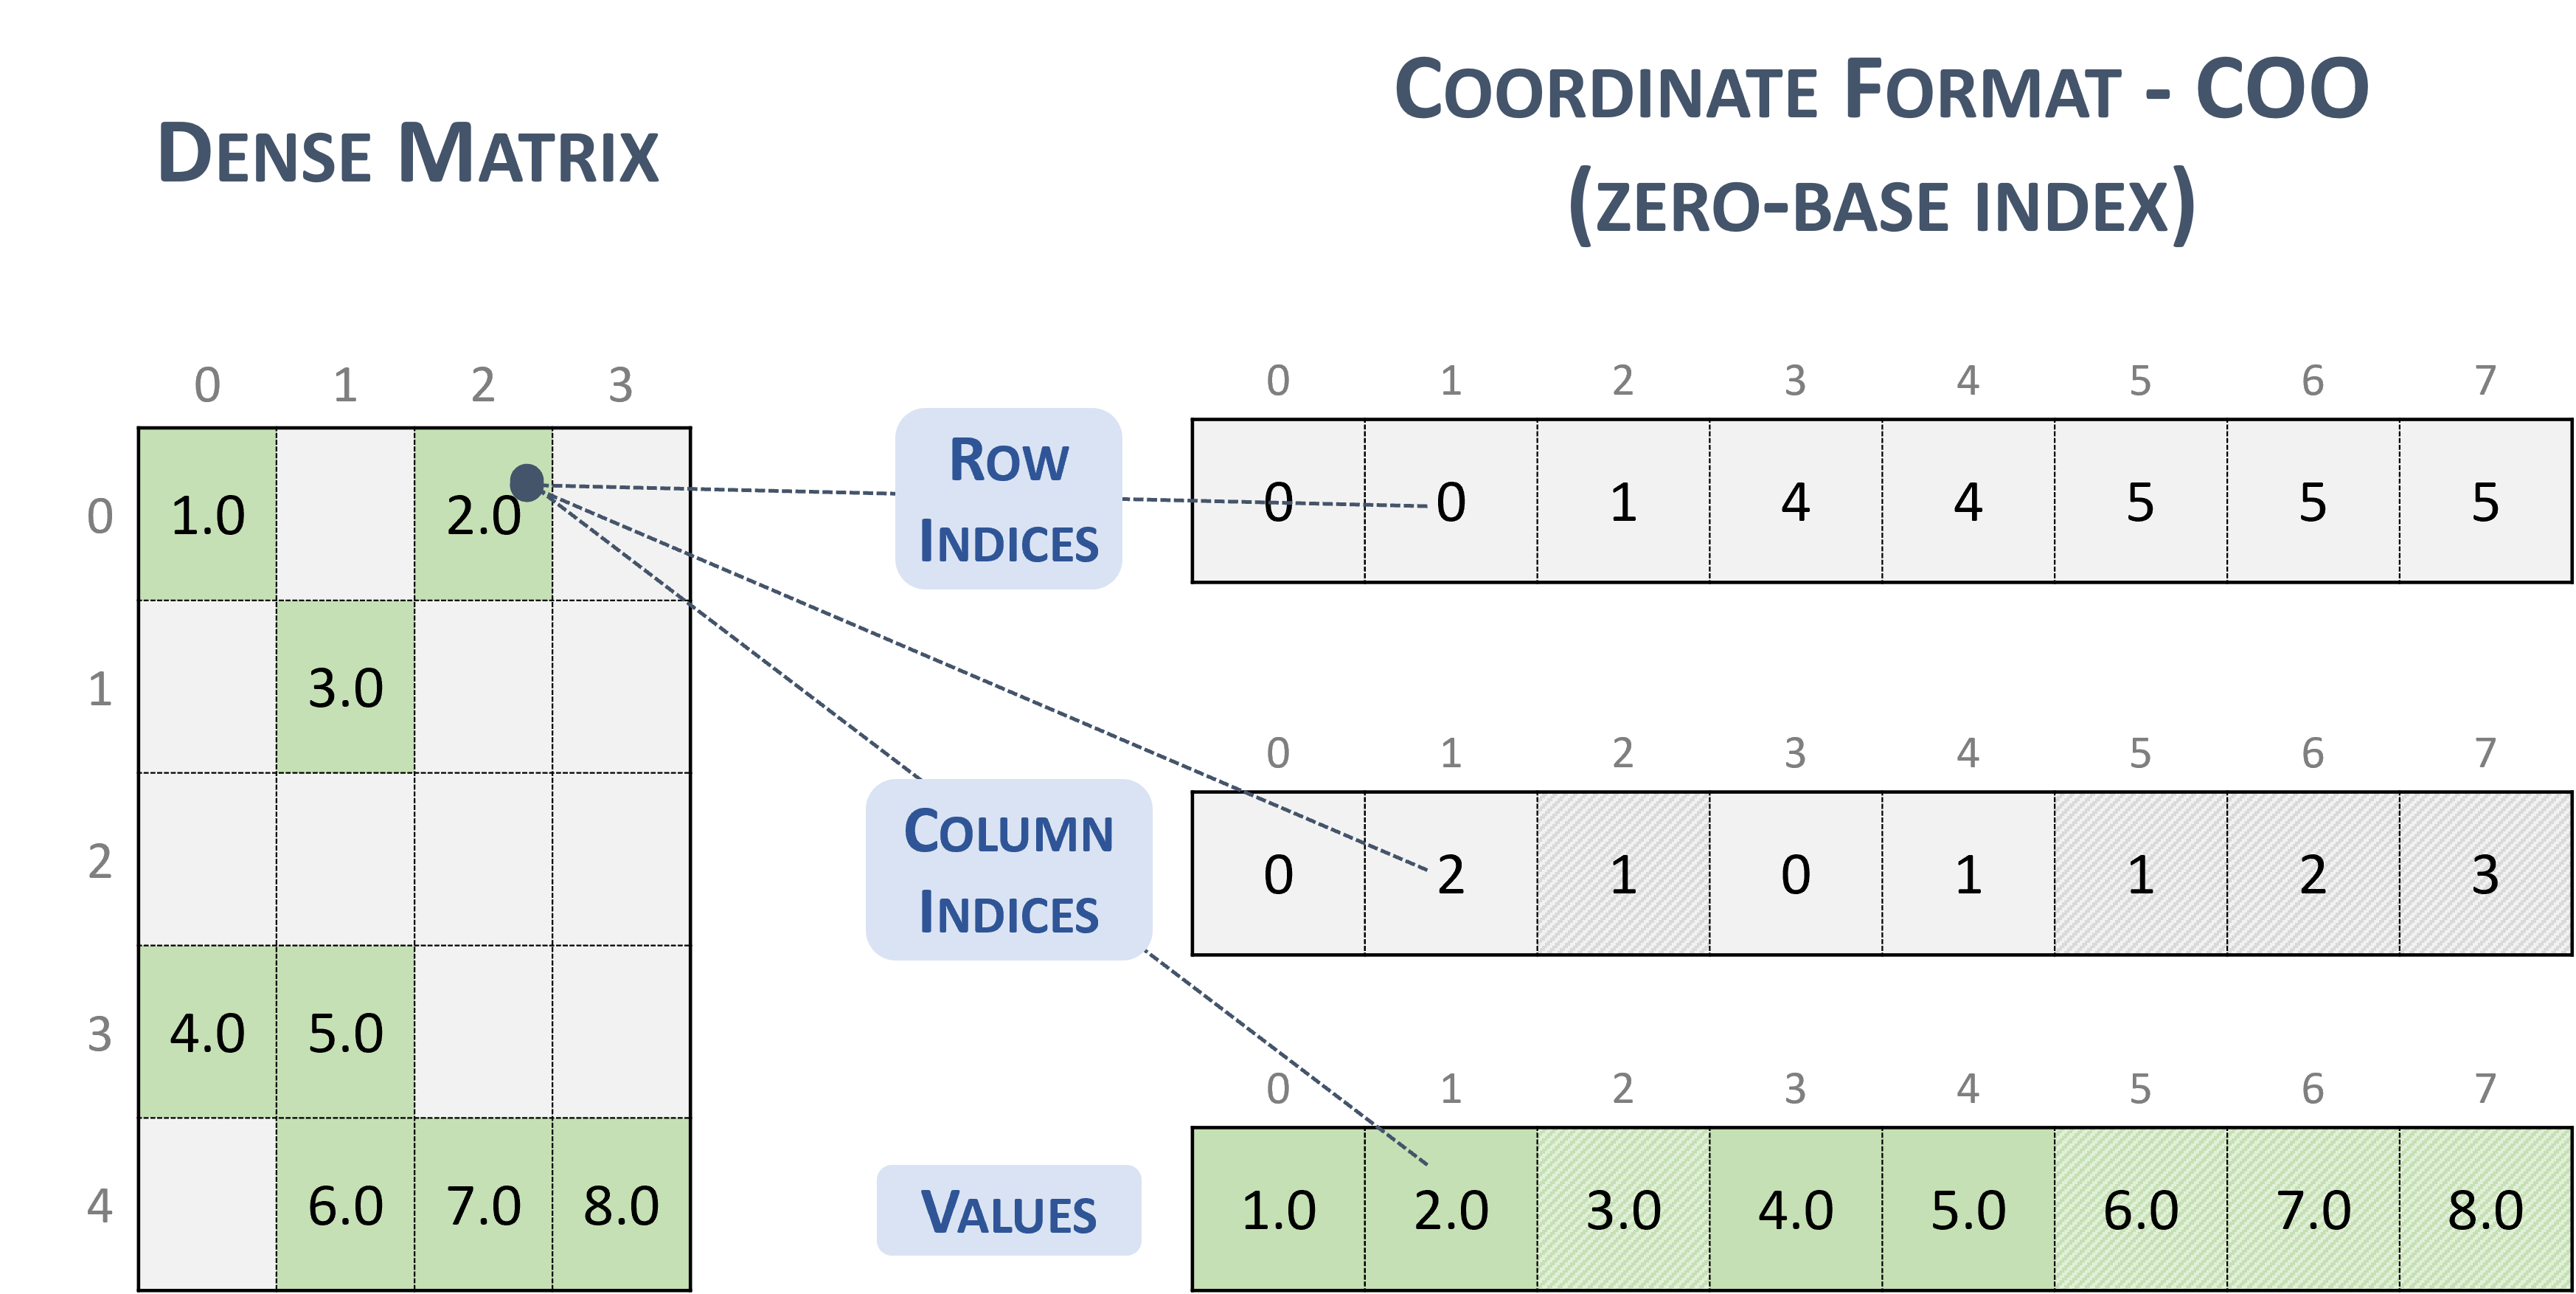
\includegraphics[width=\textwidth]{img/coo.png}
		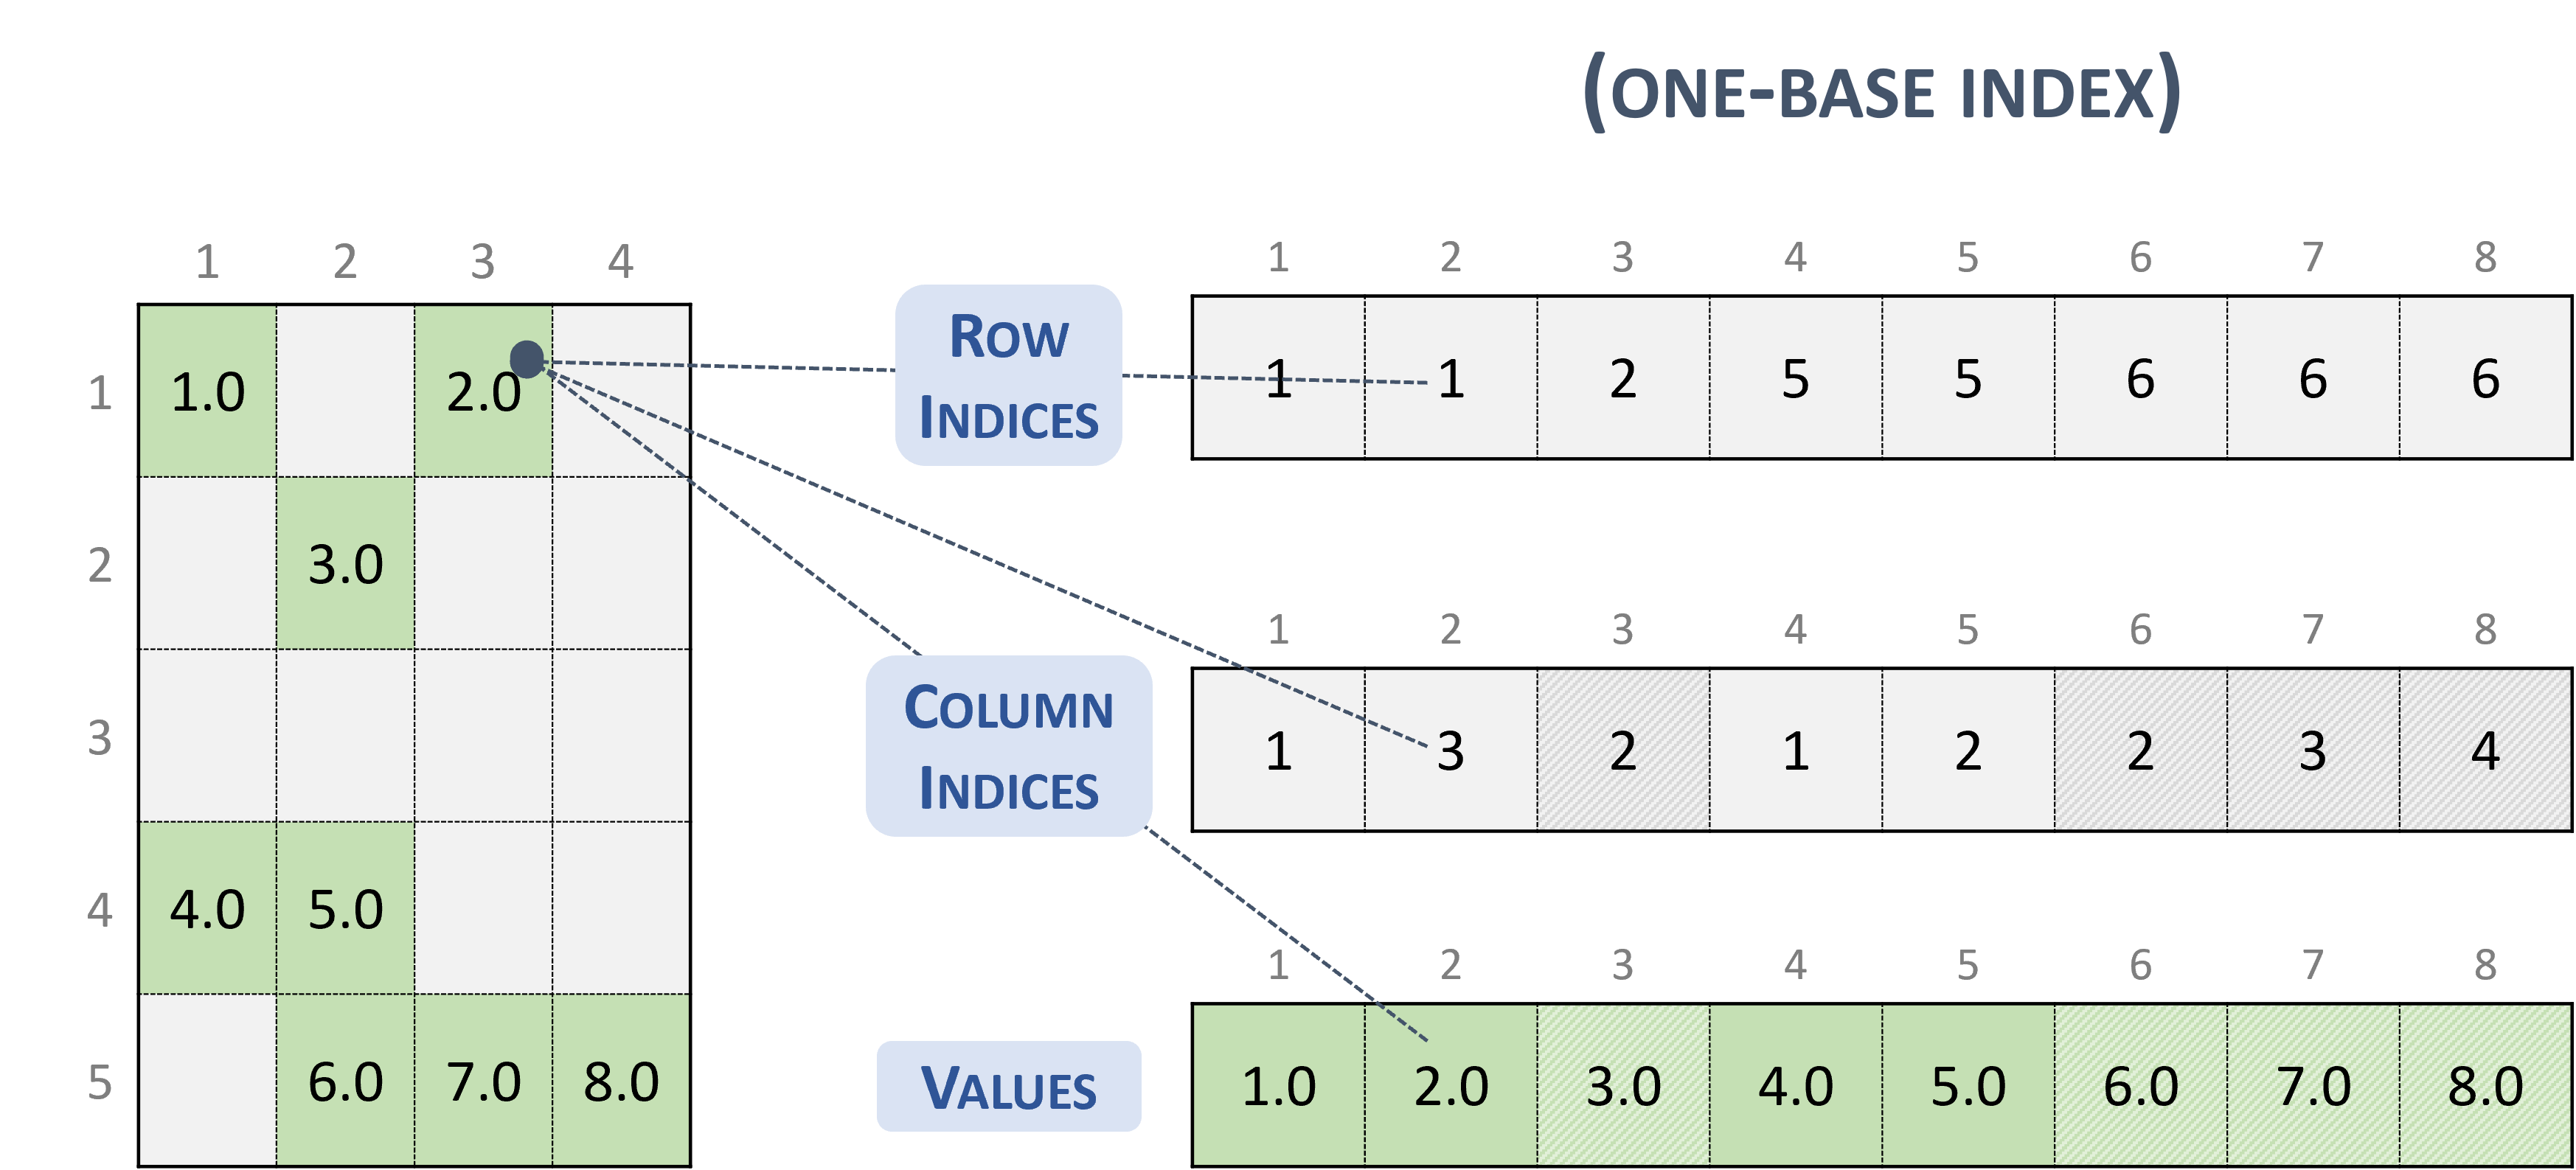
\includegraphics[width=\textwidth]{img/coo_one_base.png}
		\caption{Graphical representation of the coordinate format (COO) technique. From the figure we can see the representation of the \texttt{AA} array, called \emph{values}, the \texttt{JR}, called \emph{row indices}, and finally the \texttt{JC}, called \emph{column indices}. The algorithm is very simple. The figures are taken from the \href{https://docs.nvidia.com/nvpl/_static/sparse/storage_format/sparse_matrix.html}{NVIDIA Performance Libraries Sparse}, which is part of the \href{https://developer.nvidia.com/nvpl}{NVIDIA Performance Libraries}.}
	\end{figure}
	
	\item \definition{Coordinate Compressed Sparse Row format (CSR)}. If the elements of $A$ are listed by row, the array \texttt{JC} might be replaced by an array that points to the beginning of each row.
	\begin{itemize}
		\item \texttt{AA}: all the values of the non-zero elements of $A$, stored row by row from $1, \dots, n$.
		
		\item \texttt{JA}: contains the column indices.
		
		\item \texttt{IA}: contains the pointers to the beginning of each row in the arrays $A$ and \texttt{JA}. Thus \texttt{IA}$\left(i\right)$ contains the position in the arrays \texttt{AA} and \texttt{JA} where the $i$-th row starts. The length of \texttt{IA} is $n+1$, with $\texttt{IA}\left(n+1\right)$ containing the number $A\left(1\right) + \nnz\left(A\right)$. Remember that $n$ is the number of rows.
	\end{itemize}
	For \example{example}:
	\begin{equation*}
		A = \begin{bmatrix}
			1. & 0. & 0.& 2. & 0. \\
			3. & 4. & 0.& 5. & 0. \\
			6. & 0. & 7.& 8. & 9. \\
			0. & 0. & 10.& 11. & 0. \\
			0. & 0. & 0.& 0. & 12. 
		\end{bmatrix}
	\end{equation*}
	\begin{equation*}
		\begin{array}{rcl}
			\texttt{AA} &=& \left[
				1.\hspace{1em}
				2.\hspace{1em}
				3.\hspace{1em}
				\phantom{1}4.\hspace{1em}
				\phantom{1}5.\hspace{1em}
				\phantom{1}6.\hspace{1em}
				7.\hspace{1em}
				8.\hspace{1em}
				9.\hspace{1em}
				10.\hspace{1em}
				11.\hspace{1em}
				12.
			\right] \\ [.5em]
			\texttt{JA} &=& \left[
				1\phantom{.}\hspace{1em}
				4\phantom{.}\hspace{1em}
				1\phantom{.}\hspace{1em}
				\phantom{1}2\phantom{.}\hspace{1em}
				\phantom{1}4\phantom{.}\hspace{1em}
				\phantom{1}1\phantom{.}\hspace{1em}
				3\phantom{.}\hspace{1em}
				4\phantom{.}\hspace{1em}
				5\phantom{.}\hspace{1em}
				\phantom{1}3\phantom{.}\hspace{1em}
				\phantom{1}4\phantom{.}\hspace{1em}
				\phantom{1}5\phantom{.}
			\right] \\ [.5em]
			\texttt{IA} &=& \left[
				1\phantom{.}\hspace{1em}
				3\phantom{.}\hspace{1em}
				6\phantom{.}\hspace{1em}
				10\phantom{.}\hspace{1em}
				12\phantom{.}\hspace{1em}
				13\phantom{.}
			\right]
		\end{array}
	\end{equation*}
	To retrieve each position of the matrix, the algorithm is quite simple. Consider the \texttt{IA} arrays. 
	\begin{enumerate}
		\item We start at position one of the array, then the value 1:
		\begin{equation*}
			\begin{array}{rcl}
				\texttt{AA} &=& \left[
				1.\hspace{1em}
				2.\hspace{1em}
				3.\hspace{1em}
				\phantom{1}4.\hspace{1em}
				\phantom{1}5.\hspace{1em}
				\phantom{1}6.\hspace{1em}
				7.\hspace{1em}
				8.\hspace{1em}
				9.\hspace{1em}
				10.\hspace{1em}
				11.\hspace{1em}
				12.
				\right] \\ [.5em]
				\texttt{JA} &=& \left[
				1\phantom{.}\hspace{1em}
				4\phantom{.}\hspace{1em}
				1\phantom{.}\hspace{1em}
				\phantom{1}2\phantom{.}\hspace{1em}
				\phantom{1}4\phantom{.}\hspace{1em}
				\phantom{1}1\phantom{.}\hspace{1em}
				3\phantom{.}\hspace{1em}
				4\phantom{.}\hspace{1em}
				5\phantom{.}\hspace{1em}
				\phantom{1}3\phantom{.}\hspace{1em}
				\phantom{1}4\phantom{.}\hspace{1em}
				\phantom{1}5\phantom{.}
				\right] \\ [.5em]
				\texttt{IA} &=& \left[
				\circledtext{1}\phantom{.}\hspace{.4em}
				3\phantom{.}\hspace{1em}
				6\phantom{.}\hspace{1em}
				10\phantom{.}\hspace{1em}
				12\phantom{.}\hspace{1em}
				13\phantom{.}
				\right]
			\end{array}
		\end{equation*}
		
		
		\item We use the value one to see the first (index one) position of the array JA, and the value is 1:
		\begin{equation*}
			\begin{array}{rcl}
				\texttt{AA} &=& \left[
				1.\hspace{1em}
				2.\hspace{1em}
				3.\hspace{1em}
				\phantom{1}4.\hspace{1em}
				\phantom{1}5.\hspace{1em}
				\phantom{1}6.\hspace{1em}
				7.\hspace{1em}
				8.\hspace{1em}
				9.\hspace{1em}
				10.\hspace{1em}
				11.\hspace{1em}
				12.
				\right] \\ [.5em]
				\texttt{JA} &=& \left[
				\circledtext{1}\phantom{.}\hspace{.4em}
				4\phantom{.}\hspace{1em}
				1\phantom{.}\hspace{1em}
				\phantom{1}2\phantom{.}\hspace{1em}
				\phantom{1}4\phantom{.}\hspace{1em}
				\phantom{1}1\phantom{.}\hspace{1em}
				3\phantom{.}\hspace{1em}
				4\phantom{.}\hspace{1em}
				5\phantom{.}\hspace{1em}
				\phantom{1}3\phantom{.}\hspace{1em}
				\phantom{1}4\phantom{.}\hspace{1em}
				\phantom{1}5\phantom{.}
				\right] \\ [.5em]
				\texttt{IA} &=& \left[
				1\phantom{.}\hspace{1em}
				3\phantom{.}\hspace{1em}
				6\phantom{.}\hspace{1em}
				10\phantom{.}\hspace{1em}
				12\phantom{.}\hspace{1em}
				13\phantom{.}
				\right]
			\end{array}
		\end{equation*}
		
		\item But with the same index of \texttt{IA}, you also check the array \texttt{AA}, which has a value of 1:
		\begin{equation*}
			\begin{array}{rcl}
				\texttt{AA} &=& \left[
				\circledtext{1.}\hspace{.6em}
				2.\hspace{1em}
				3.\hspace{1em}
				\phantom{1}4.\hspace{1em}
				\phantom{1}5.\hspace{1em}
				\phantom{1}6.\hspace{1em}
				7.\hspace{1em}
				8.\hspace{1em}
				9.\hspace{1em}
				10.\hspace{1em}
				11.\hspace{1em}
				12.
				\right] \\ [.5em]
				\texttt{JA} &=& \left[
				1\phantom{.}\hspace{1em}
				4\phantom{.}\hspace{1em}
				1\phantom{.}\hspace{1em}
				\phantom{1}2\phantom{.}\hspace{1em}
				\phantom{1}4\phantom{.}\hspace{1em}
				\phantom{1}1\phantom{.}\hspace{1em}
				3\phantom{.}\hspace{1em}
				4\phantom{.}\hspace{1em}
				5\phantom{.}\hspace{1em}
				\phantom{1}3\phantom{.}\hspace{1em}
				\phantom{1}4\phantom{.}\hspace{1em}
				\phantom{1}5\phantom{.}
				\right] \\ [.5em]
				\texttt{IA} &=& \left[
				1\phantom{.}\hspace{1em}
				3\phantom{.}\hspace{1em}
				6\phantom{.}\hspace{1em}
				10\phantom{.}\hspace{1em}
				12\phantom{.}\hspace{1em}
				13\phantom{.}
				\right]
			\end{array}
		\end{equation*}
		
		\item Now we can check the next row of the matrix. So we check the array \texttt{IA} at position 2 and get the value 3. But be careful! From 1 (the previously calculated value) to 3 (the value just taken) there is the value 2 in between. So we can assume that the value 2 is also in the first row.
		\begin{equation*}
			\begin{array}{rcl}
				\texttt{AA} &=& \left[
				1.\hspace{1em}
				\circledtext{2.}\hspace{.6em}
				3.\hspace{1em}
				\phantom{1}4.\hspace{1em}
				\phantom{1}5.\hspace{1em}
				\phantom{1}6.\hspace{1em}
				7.\hspace{1em}
				8.\hspace{1em}
				9.\hspace{1em}
				10.\hspace{1em}
				11.\hspace{1em}
				12.
				\right] \\ [.5em]
				\texttt{JA} &=& \left[
				1\phantom{.}\hspace{1em}
				\circledtext{4}\phantom{.}\hspace{.4em}
				1\phantom{.}\hspace{1em}
				\phantom{1}2\phantom{.}\hspace{1em}
				\phantom{1}4\phantom{.}\hspace{1em}
				\phantom{1}1\phantom{.}\hspace{1em}
				3\phantom{.}\hspace{1em}
				4\phantom{.}\hspace{1em}
				5\phantom{.}\hspace{1em}
				\phantom{1}3\phantom{.}\hspace{1em}
				\phantom{1}4\phantom{.}\hspace{1em}
				\phantom{1}5\phantom{.}
				\right] \\ [.5em]
				\texttt{IA} &=& \left[
				1\phantom{.}\hspace{1.3em}
				3\phantom{.}\hspace{.7em}
				6\phantom{.}\hspace{1em}
				10\phantom{.}\hspace{1em}
				12\phantom{.}\hspace{1em}
				13\phantom{.}
				\right]
			\end{array}
		\end{equation*}
	\end{enumerate}
	\newpage
	\begin{figure}[!htp]
		\centering
		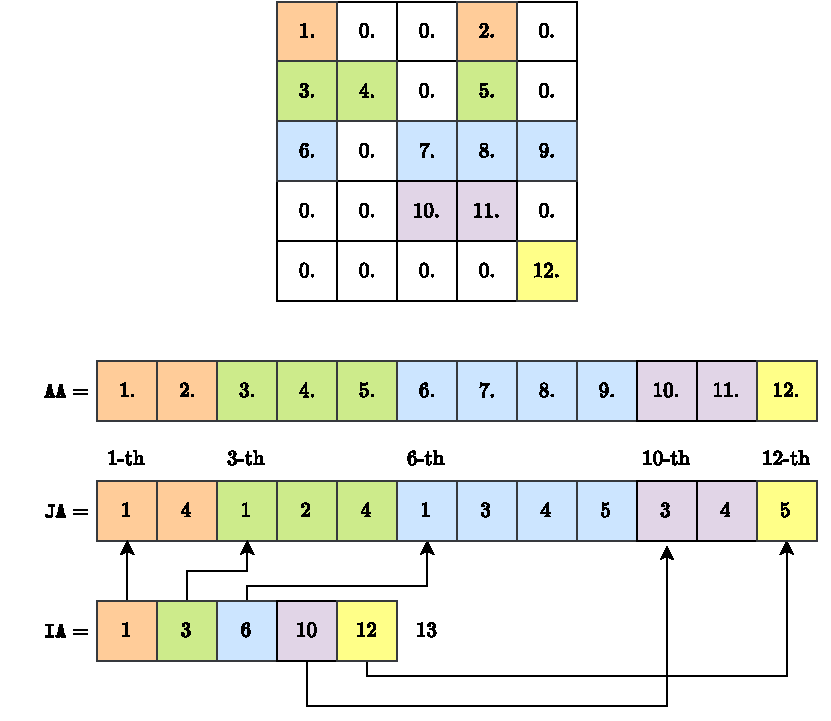
\includegraphics[width=\textwidth]{img/crs.pdf}
		\caption{View an illustration of the CRS technique using colors to improve readability.}
	\end{figure}
	\begin{figure}[!htp]
		\centering
		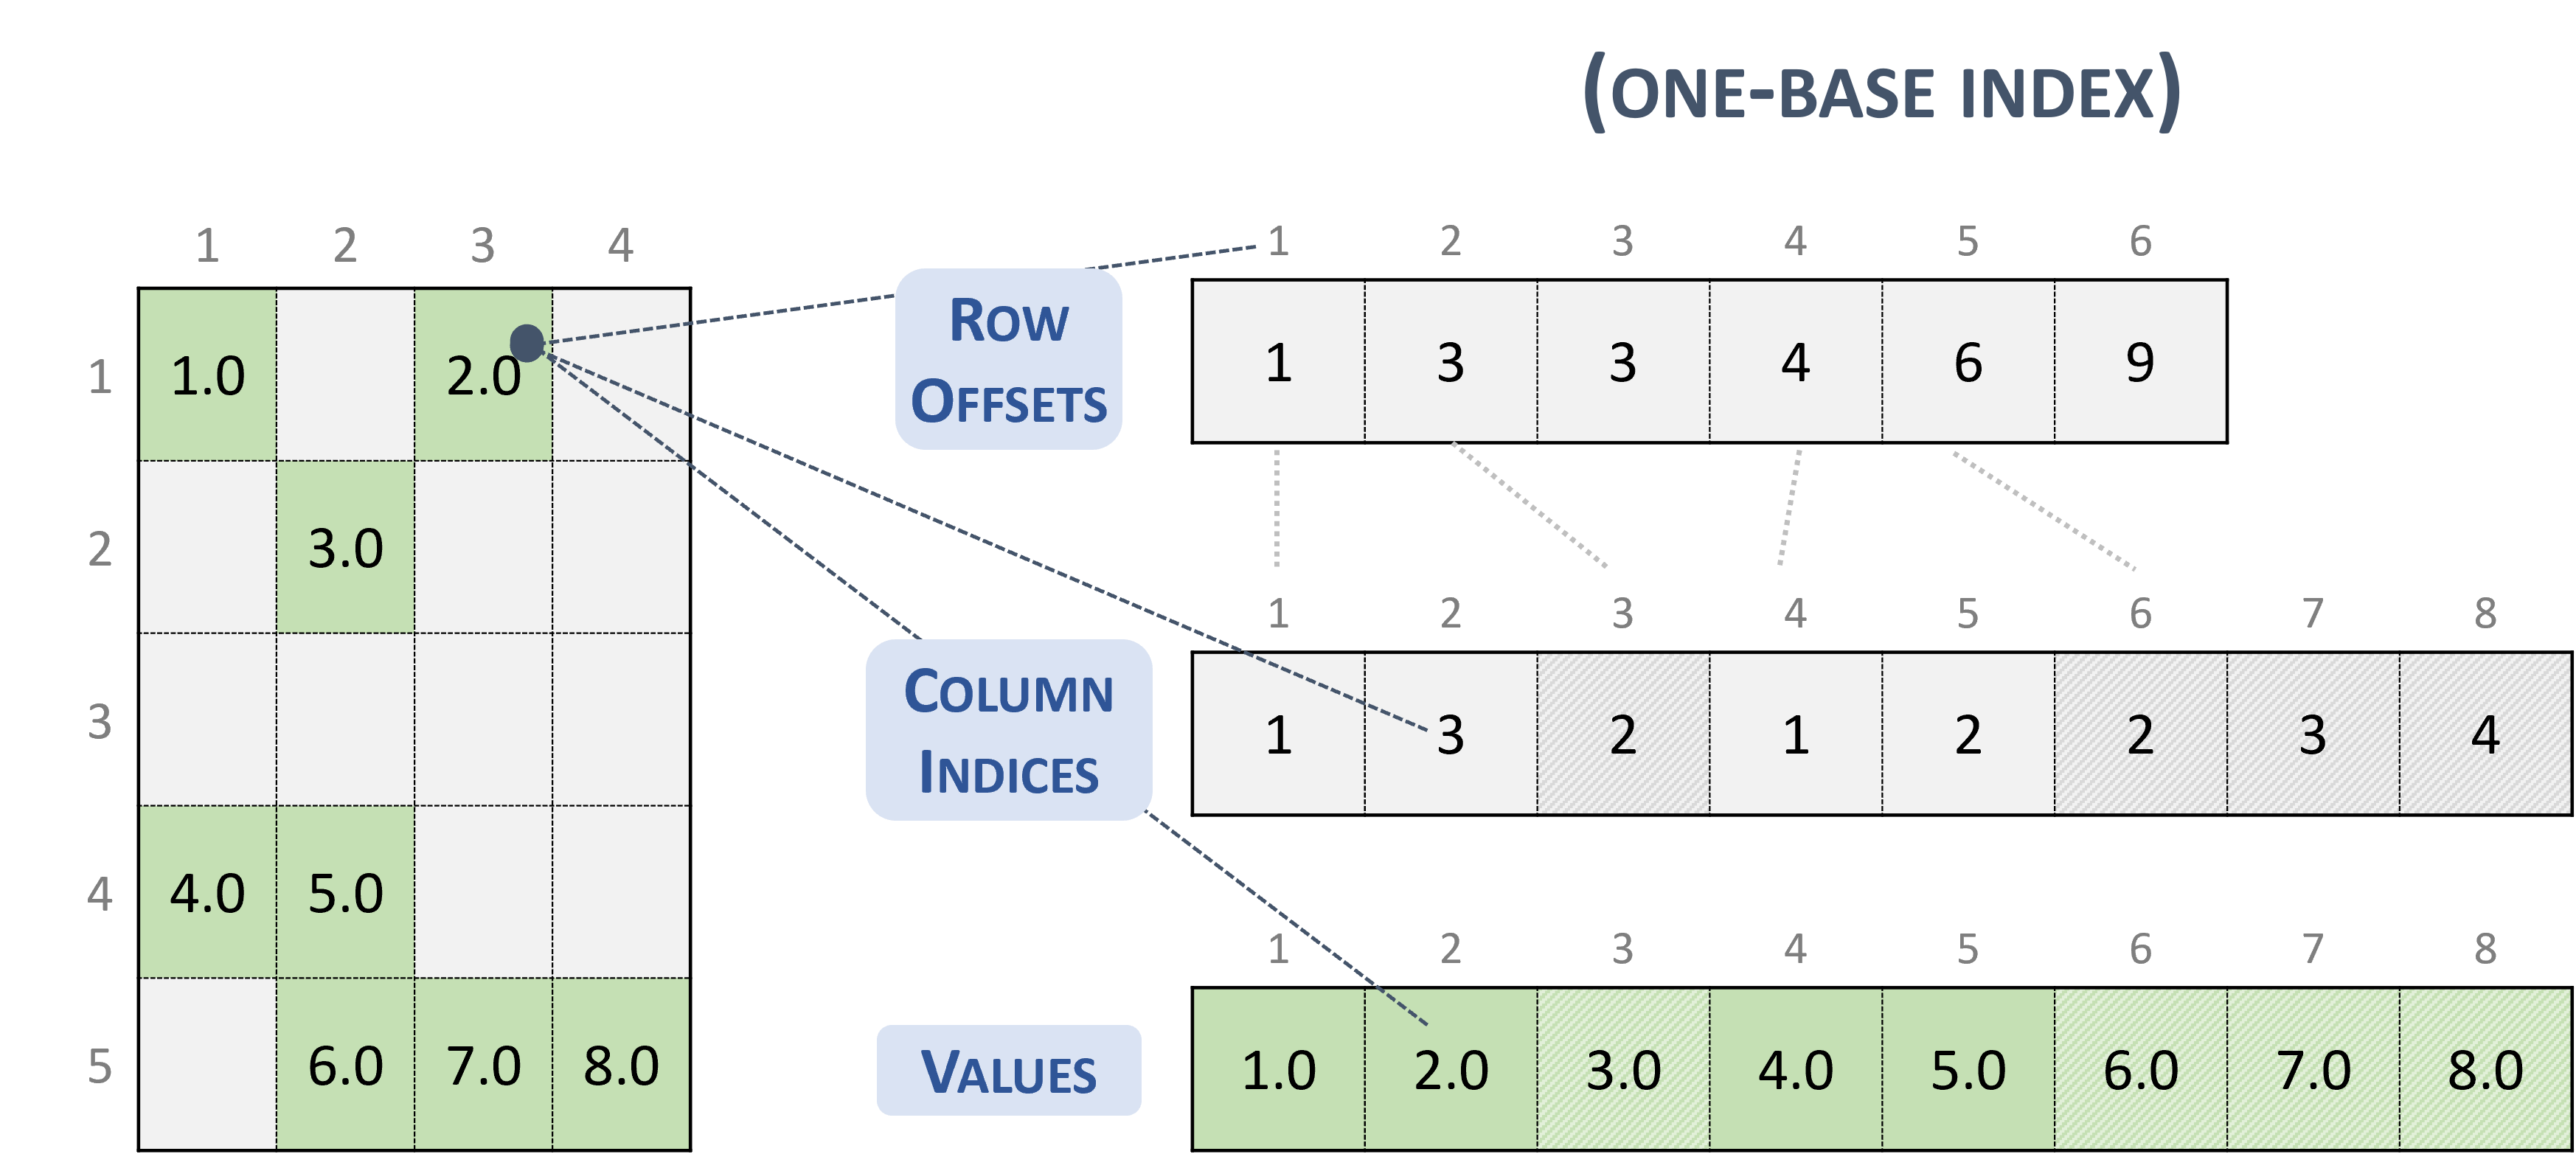
\includegraphics[width=.9\textwidth]{img/csr_one_base.png}
		\caption{Graphical representation of the coordinate compressed sparse row (CSR) technique. From the figure we can see the representation of the \texttt{AA} array, called \emph{values}, the \texttt{IA}, called \emph{row offset}, and finally the \texttt{JA}, called \emph{column indices}.
		It's interesting to see how the empty line case is handled. It copies the previous value of the array.
		The figures are taken from the \href{https://docs.nvidia.com/nvpl/_static/sparse/storage_format/sparse_matrix.html}{NVIDIA Performance Libraries Sparse}, which is part of the \href{https://developer.nvidia.com/nvpl}{NVIDIA Performance Libraries}.}
	\end{figure}
\end{itemize}